\documentclass{article}
\usepackage{amssymb}
\usepackage{amsmath}
\usepackage{amsthm}
\usepackage{mathtools}
\usepackage{hyperref}
\usepackage{float}
\usepackage{graphicx} % Required for inserting images
\usepackage{tikz}
\usepackage{multicol}
\usetikzlibrary{fit}
\newcommand{\overlay}[2][]{\tikz[overlay,
  remember picture, #1]{#2}}
\tikzset{
  highlighted/.style = { draw, thick, rectangle,
                         rounded corners, inner sep = 0pt,
                         fill = red!15, fill opacity = 0.5
                       }
}
\newcommand{\highlight}[1]{%
  \overlay{
    \node [fit = (left.north west) (right.south east),
           highlighted] (#1) {}; }
}
\newcommand{\flag}[2]{\overlay[baseline=(#1.base)]
  {\node (#1) {$#2$};}}

% TODO
% implementing in python the kronecker operator
% also the vec operator
% try to replicate fact1
% checking the np-complete and np-hard problems
% 

\newtheorem{theorem}{Theorem}[section]
\newtheorem{corollary}{Corollary}[theorem]
\newtheorem{lemma}[theorem]{Lemma}

\title{Autoencoders explained}
\author{Lorenzo Bozzoni}
\date{March 2024}

\begin{document}

\maketitle
\tableofcontents

\section{Introduction}
Autoencoders are simple learning circuits which aim to transform inputs into outputs with
the least possible amount of distortion. To derive a fairly general framework, an $n/p/n$  autoencoder is defined by a t-uple $n,p,m,\mathbb{F},\mathbb{G},\mathcal{A},\mathcal{B},\mathcal{X},\mathcal{Y}, \Delta$, where:
\begin{itemize}
    \item $\mathbb{F}$ and $\mathbb{G}$ are sets
    \item $n$ and $p$ are positive integers
    \item $\mathcal{A}$ is a class of functions from $\mathbb{G}^p$ to $\mathbb{F}^n$
    \item $\mathcal{B}$ is a class of functions from $\mathbb{F}^n$ to $\mathbb{G}^p$
    \item $\mathcal{X} = {x_1, \dots, x_m}$ is a set of $m$ (training) vectors in $\mathbb{F}^n$. When the external targets are present, we let $\mathcal{Y} = {y_1, \dots, y_m}$ denote the corresponding set of $m$ target vectors in $\mathbb{F}^n$ 
    \item $\Delta$ is a dissimilarity or distortion function defined over $\mathbb{F}^n$
\end{itemize}
For any $A \in \mathcal{A}$ and $B \in \mathcal{B}$, the autoencoder transforms an input vector $x \in \mathbb{F}^n$ into an output vector $A \circ B(x) \in \mathbb{F}^n$. The corresponding \textbf{autoencoder problem} is to find $A \in \mathcal{A}$ and $B \in \mathcal{B}$ that minimize the overall distortion function:
\begin{equation}
    \min E(A,B) = \min_{A ,B} \sum_{t=1}^m E(A,B)=\min_{A ,B} \sum_{t=1}^m \Delta(x_t, A \circ B(x_t))
\end{equation}
In the non auto-associative case, when external targets $y_t$ are provided, the minimization
problem becomes:
\begin{equation}
    \min E(A,B) = \min_{A ,B} \sum_{t=1}^m E(A,B)=\min_{A ,B} \sum_{t=1}^m \Delta(y_t, A \circ B(x_t))
\end{equation}
It is important to notice that if $p < n$ corresponds to a compression or feature extraction, while $p > n$ corresponds to a decompression. 

\section{Linear Autoencoders}
We consider the problem of learning from examples in layered linear feed-forward neural networks using optimization methods, such as back propagation, with respect to the usual quadratic error function E of the connection weights. 

We assume to have $N$ samples and $N$ lables so for each $x_n$ input vector corresponds the $y_n$ label. The classical quadratic error function is defined as:
\[
E = \sum_{t=1}^m \|y_t - F(x_t)\|^2 
\]
where $F$ is the current function implemented by the network. We defined also the \textbf{covariance matrices}:
\[
\begin{split}
    \Sigma_{XX} &= \sum_{t=1}^m x_t x_t^\intercal \hspace{1cm} \Sigma_{YX} = \sum_{t=1}^m y_t x_t^\intercal\\
    \Sigma_{YY} &= \sum_{t=1}^m y_t y_t^\intercal \hspace{1cm} \Sigma_{XY} = \sum_{t=1}^m x_t y_t^\intercal
\end{split}
\]
Where these quantities are defined. \\

Of course the aim is not trivially to minimize the error function, since this would be simply solved by choosing as global mapping $W = AB = I$, but rather to find $W$ such that, having a smaller rank, it performs a good compression of the input data.

\subsection{Useful mathematical concepts}
For any matrices $P, Q, R$ we have $tr(PQR) = tr(RPQ) = tr(QRP)$ provided that these quantities are defined. Thus in particolar if $P$ is \textbf{idempotent}, that is, $P^2 = P$, then:
\begin{equation}\tag{a}
    tr(PQP) = tr(PPQ) = tr(P^2Q) = tr(PQ)
\end{equation}
If $U$ is orthogonal, that is $U^\intercal U = I$, then:
\begin{equation}\tag{b}
    tr(UQU^\intercal) = tr(U^\intercal UQ) = tr(Q)
\end{equation}

The \textbf{Kronecker product} $P \otimes Q$ of any two matrices $P$ and $Q$ is the matrix obtained from the matrix $P$ by replacing each entry $p_{ij}$ of $P$ with the matrix $p_{ij}Q$. Which means that:
\[P: m\times n \text{ and } Q:r\times q \implies 
P \otimes Q = \begin{bmatrix}
    p_{11}Q & \dots & a_{1n}Q\\
    \vdots & \ddots & \vdots\\
    p_{m1}Q & \dots & p_{mn}Q\\
\end{bmatrix}
\text{ of shape } rm\times qn
\]
The \textbf{vec operation} transforms a matrix into a column vector by stacking the columns of the matrix one underneath the other. Indeed, if $P$ is any $m \times n$ matrix and $p_j$ is the $j$-th column, then $vec(P)$ is the $mn\times 1$ vector $vec(P) = [p_1^\intercal, \dots, p_n^\intercal]^\intercal$.

We have that:
\begin{equation} \tag{c}
    tr(PQ^\intercal) = (vec(P))^\intercal vec(Q)
\end{equation}

\begin{equation} \tag{d}
    vec(PQR^\intercal) = (R \otimes P) vec(Q)
\end{equation}

\begin{equation} \tag{e}
    (P \otimes Q)(R \otimes S) = PR \otimes QS
\end{equation}

\begin{equation} \tag{f}
    (P \otimes Q)^{-1} = P^{-1} \otimes Q^{-1}
\end{equation}

\begin{equation} \tag{g}
    (P \otimes Q)^\intercal = P^\intercal \otimes Q^\intercal
\end{equation}
whenever these quantities are defined. Also: if $P$ and $Q$ are symmetric and positive semidefinite (resp. definite) then $P \otimes Q$ is symmetric and positive semidefinite (resp. positive definite) (h).

Finally, let us introduce the input data matrix $X = [x_1, \dots, x_N]$ and the output data matrix $Y=[y_1, \dots, y_N]$. It is easily seen that $XX^\intercal = \Sigma_{XX}$, $XY^\intercal = \Sigma_{XY}$, $YY^\intercal = \Sigma_{YY}$, $YX^\intercal = \Sigma_{YX}$ and $E(A,B) = \|vec(Y - ABX)\|^2$. In the proof of facts 1 and 2, we shall use the following well known lemma.

\textbf{Lemma}: the quadratic function:
\[F(z) = \|c - Mz\|^2 = c^\intercal c - 2c^\intercal Mz + z^\intercal M^\intercal M z\]
is convex. A point $z$ corresponds to a global minimum of $F$ if and only if it satisfies the equation $\nabla F = 0$, or equivalently $M^\intercal M z = M^\intercal c$. If in addition $M^\intercal M$ is positive definite, then $F$ is strictly convex and the unique minimum of $F$ is attained for $z = (M^\intercal M)^{-1} M^\intercal c$.
    

\subsection{Fact 1}
For any fixed $n \times p$ matrix $A$ the function $E(A,B)$ is convex in the coefficients of $B$ and attains its minimum for any $B$ satisfying the equation
\begin{equation}
    A^\intercal AB\Sigma_{XX} = A^\intercal \Sigma_{YX}
\end{equation}
If $\Sigma_{XX}$ is invertible and A is full rank $p$, then $E$ is strictly convex and has unique minimum reached when:
\begin{equation}\tag{3}
    B = \hat{B}(A) = (A^\intercal A)^{-1} A^\intercal \Sigma_{YX}\Sigma_{XX}^{-1}
\end{equation}
In the auto-associative case, (3) becomes 
\begin{equation}\tag{3'}
    B = \hat{B}(A) = (A^\intercal A)^{-1} A^\intercal 
\end{equation}
Since $Y=X$ so $\Sigma_{YX}\Sigma_{XX}^{-1} = I$.

\subsubsection{Proof of fact 1}
\begin{proof}
    For fixed A, use (d) to write:
    \[
        vec(Y - ABX) = vec(Y) - vec(ABX) = vec(Y) - (X^\intercal \otimes A) vec(B)
    \]
    and thus:
    \[
    E(A,B) = \|vec(Y) - (X^\intercal \otimes A) vec(B)\|^2
    \]
    By the above lemma, $E$ is convex in the coefficients of B and B corresponds to a global minimum if and only if \[
    (X^\intercal \otimes A)^\intercal (X^\intercal \otimes A) vec(B) = (X^\intercal \otimes A) vec(Y)
    \]
    Now on one hand:
    \[
    \begin{split}
         (X^\intercal \otimes A)^\intercal (X^\intercal \otimes A) vec(B) &= (X^\intercal \otimes A) vec(B)\\ &= (XX^\intercal \otimes A^\intercal A) vec(B)\\ &= (\Sigma_{XX} \otimes A^\intercal A)vec(B) \\ &= vec(A^\intercal A B\Sigma_{XX})
    \end{split}
    \]
    On the other hand:
    \[
        \begin{split}
            (X^\intercal \otimes A)^\intercal vec(Y) &= (X \otimes A^\intercal)vec(Y) \\
            &= vec(A^\intercal YX^\intercal)\\
            &= vec(A^\intercal \Sigma_{YX})
        \end{split}
    \]
    Therefore:
    \[
        A^\intercal AB\Sigma_{XX} = A^\intercal \Sigma_{YX}
    \]
    which is (2). If $A$ is full rank, $A^\intercal A$ is symmetric and positive definite. As a covariance matrix, $\Sigma_{XX}$ is symmetric and positive semidefinite; if, in addition, $\Sigma_{XX}$ is invertible, then $\Sigma_{XX}$ is also positive definite. Because of (h), $(X^\intercal  \otimes A)^\intercal (X^\intercal \otimes A) = \Sigma_{XX} \otimes A^\intercal A$ is also symmetric and positive definite. Applying the above lemma, we conclude that if $\Sigma_{XX}$ is invertible and A is a fixed full rank matrix, then $E$ is strictly convex in the coefficients of $B$ and attains its unique minimum at the unique solution $B = \hat{B}(A) = (A^\intercal A)^{-1}A^\intercal \Sigma_{YX} \Sigma_{XX}^{-1}$ of (2), which is (3). In the auto-associative case, $x_n = y_n$. Therefore $\Sigma_{XX} = \Sigma_{YX} = \Sigma_{YY} = \Sigma_{XY}$ and the above expression simplifies to (3').
    \end{proof}

\subsection{Fact 2}
For any fixed $p \times n$ matrix $B$ the function $E(A,B)$ is convex in the coefficients of $A$ and attains its minimum for any $A$ satisfying the equation:
\begin{equation} \tag{4}
    AB\Sigma_{XX}B^\intercal= \Sigma_{YX}B^\intercal 
\end{equation}
If $\Sigma_{XX}$ is invertible and $B$ is full rank $p$, then $E$ is strictly convex and has a unique minimum reached when:
\begin{equation} \tag{5}
    A = \hat{A}(B) = \Sigma_{YX}B^\intercal (B\Sigma_{XX}B^\intercal)^{-1}
\end{equation}
In the auto-associative case, (5) becomes:
\begin{equation} \tag{5'}
    A = \hat{A}(B) = \Sigma_{XX}B^\intercal (B\Sigma_{XX}B^\intercal)^{-1}
\end{equation}
The proof is nearly identical to the proof of fact 1.




\subsection{Fact 3}
Assume that $\Sigma_{XX}$ is invertible. If two matrices $A$ and $B$ define a critical point of $E$ (i.e. a point where $\frac{\partial E}{\partial a_{ij}} = \frac{\partial E}{\partial b_{ij}} = 0$) then the global map $W = AB$ is of the form:
\begin{equation} \tag{6}
    W = P_A \Sigma_{YX}\Sigma_{XX}^{-1}
\end{equation}
with $A$ satisfying
\begin{equation} \tag{7}
    P_A \Sigma = P_A \Sigma P_A = \Sigma P_A    
\end{equation}
Where $\Sigma = \Sigma_{YX} \Sigma_{XX}^{-1} \Sigma_{XY}$. Recall also, that the matrix $P_A$ is the matrix of the orthogonal projection onto the subspace spanned by the columns of $A$. In the auto-associative case, $\Sigma = \Sigma_{XX}$ and (6) and (7) become:
\begin{equation} \tag{6'}
    W = AB = P_A
\end{equation}
\begin{equation} \tag{7'}
    P_A \Sigma_{XX} = P_A \Sigma_{XX} P_A = \Sigma_{XX} P_A
\end{equation}
If $A$ is full rank $p$, then $A$ and $B$ define a critical point of $E$ if and only if $A$ satisfies (7) and $B = \hat{B}(A)$, or equivalently if and only if $A$ and $W$ satisfy (6) and (7).

\subsubsection{Proof of fact 3}
\begin{proof}
    Assume first that $A$ and $B$ define a critical point of $E$, with $A$ full rank. Then from fact 1 we get $B = \hat{B}(A)$ and thus
    \[
        W = AB = A(A^\intercal A)^{-1}A\Sigma_{YX}\Sigma_{XX}^{-1} = P_A\Sigma_{YX}\Sigma_{XX}^{-1}
    \]
    Which is (6). Multiplication of (4) by $A^\intercal$ on the right yields
    \[
        W\Sigma_{XX}W^\intercal = AB\Sigma_{XX}B^\intercal A^\intercal = \Sigma_{YX} B^\intercal A^\intercal = \Sigma_{YX} W^\intercal
    \]
    Or
    \[
        P_A\Sigma_{YX}\Sigma_{XX}^{-1}\Sigma_{XX}\Sigma_{XX}^{-1}\Sigma_{XY}P_A = \Sigma_{YX}\Sigma_{XX}^{-1}\Sigma_{XY}P_A
    \]
    Or, equivalently $P_A\Sigma P_A = \Sigma P_A$. Since both $\Sigma$ and $P_A$ are symmetric, $P_A\Sigma P_A = \Sigma P_A$ is also symmetric and therefore $\Sigma P_A = (\Sigma P_A)^\intercal = P_A^\intercal \Sigma^\intercal = P_A\Sigma$, which is (7). Hence if $A$ and $B$ correspond to a critical point and $A$ is full rank then (6) and (7) must hold and $B = \hat{B}(A)$.

    Conversely, assume that $A$ and $W$ satisfy (6) and (7), with $A$ full rank. Multiplying (6) by $(A^\intercal A)^{-1}A^\intercal$ on the left yields
    \[
        B = (A^\intercal A)^{-1}A\Sigma_{YX}\Sigma_{XX}^{-1} = \hat{B}(A)
    \]
    and (2) is satisfied. From $P_A\Sigma P_A = \Sigma P_A$ and using (6) we immediately get 
    \[
        AB\Sigma_{XX}B^\intercal A^\intercal = \Sigma_{YX}B^\intercal A^\intercal
    \]
    and multiplication of both sides by $A(A^\intercal A)^{-1}$ on the right yields 
    \[
        AB\Sigma_{XX}B^\intercal = \Sigma_{YX}B^\intercal
    \]
    which is (4). Thus $A$ and $B$ satisfy (2) and (4) and therefore they define a critical point of $E$.
\end{proof}

\subsection{Fact 4}
Assume that $\Sigma$ is full-rank with $n$ distinct eigenvalues $\lambda_1 > \dots > \lambda_n$. If $\mathcal{I} = {i_1, \dots, i_p}$ ($1 \leq i_1 < \dots < i_p \leq n$) is any ordered $p$-index set, let $U_{\mathcal{I}} = [ u_{i_1}, \dots, u_{i_p} ]$ denote the matrix formed by the orthonormal eigenvectors of $\Sigma$ associated with the eigenvalues $\lambda_{i_1}, \dots, \lambda_{i_p}$. Then two full rank matrices $A$ and $B$ define a critical point of $E$ if and only if there exist an ordered $p$-index set $\mathcal{I}$ and an invertible $p \times p$ matrix $C$ such that:
\begin{equation} \tag{8}
    A = U_{\mathcal{I}}C
\end{equation}
\begin{equation} \tag{9}
    B = C^{-1}U_{\mathcal{I}}^\intercal \Sigma_{YX}\Sigma_{XX}^{-1}
\end{equation}

For such a critical point we have:
\begin{equation} \tag{10}
    W = P_{U_\mathcal{I}}\Sigma_{YX}\Sigma_{XX}^{-1}
\end{equation}
\begin{equation} \tag{11}
    E(A,B) = tr(\Sigma_{YY}) - \sum_{i \in \mathcal{I}} \lambda_i
\end{equation}
Therefore a critical $W$ of rank $p$ is always the product of the ordinary least squares regression matrix followed by an orthogonal projection onto the subspace spanned by $p$ eigenvectors of $\Sigma$. The critical map $W$ associated with the index set $\{1,2,\dots, p\}$ is the unique local and global minimum of $E$. The remaining $\binom{n}{p} - 1$ $p$-index sets correspond to saddle points. All additional critical points defined by matrices $A$ and $B$ which are not full rank are also saddle points and can be characterized in terms of orthogonal projections onto subspaces spanned by $q$ eigenvectors of $\Sigma$ with $q < p$ (see Figure 1). 
\begin{figure}[H]
    \centering
    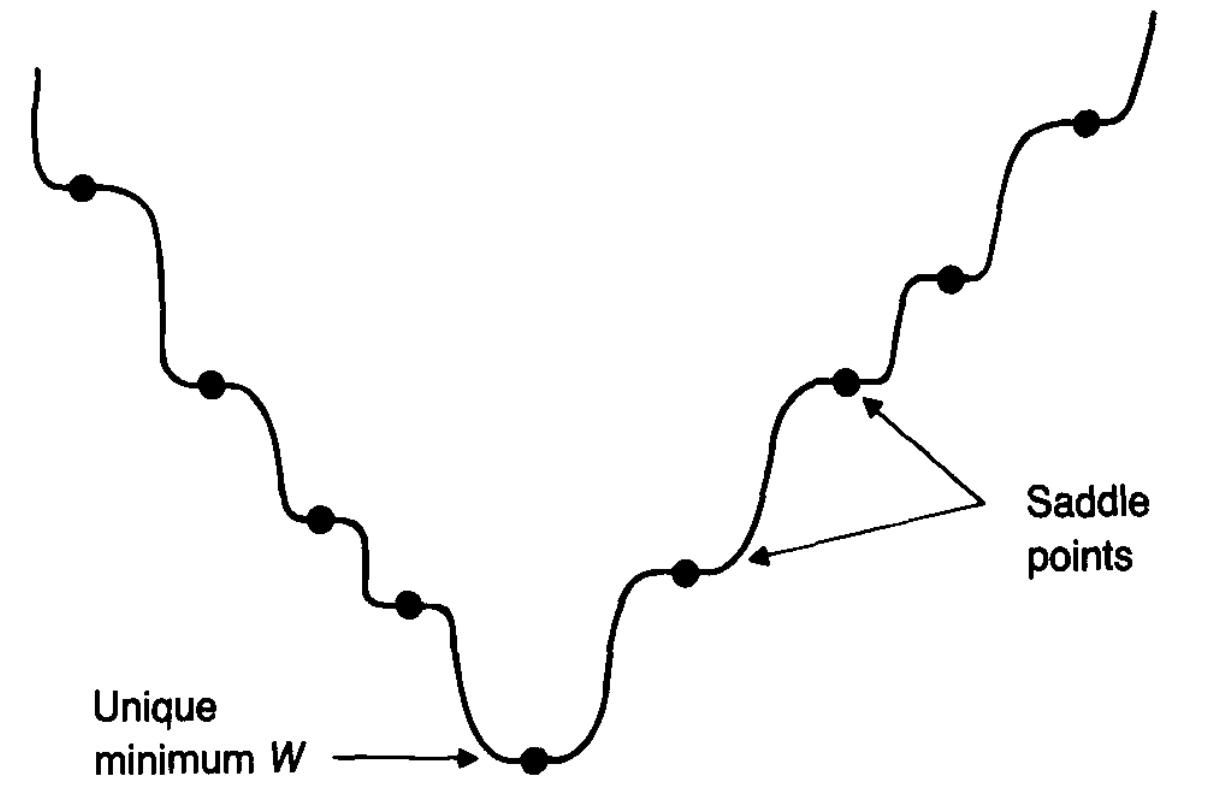
\includegraphics[width=0.5\textwidth]{./Images/LinearAutoenc_Saddles.png}
    \caption{Landscape of $E$}
    \end{figure}
In the auto-associative case, $\Sigma = \Sigma_{XX}$ and (8), (9) and (10) become:
\begin{equation} \tag{8'}
    A = U_{\mathcal{I}}C
\end{equation}
\begin{equation} \tag{9'}
    B = C^{-1}U_{\mathcal{I}}^\intercal
\end{equation}
\begin{equation} \tag{10'}
    W = P_{U_{\mathcal{I}}}
\end{equation}
and therefore the unique locally and globally optimal map $W$ is the orthogonal projection onto the subspace spanned by the first $p$ eigenvectors of $\Sigma_{XX}$ associated with the $p$ largest eigenvalues. 

\emph{Remark}: at the global minimum, if $C$ is the identity $I_p$ then the activities of the units in the hidden layer are given by:
\[
    u_1^\intercal \hat{y}_n , \dots , u_p^\intercal \hat{y}_n    
\]
the so called \textbf{principal components} of the output data $\hat{y}$. In the auto-associative case, these activities are given by $u_1^\intercal x_n, \dots, u_p^\intercal x_n$, the principal components of the input data $x$. They are the coordinates of the vector $x_n$ along the first $p$ eigenvectors of $\Sigma_{XX}$.




\subsubsection{Proof of fact 4}
First notice that since $\Sigma$ is a real symmetric covariance matrix, it can always be written as $\Sigma = U\Lambda U^\intercal$ where $U$ is an orthogonal column matrix of eigenvectors of $\Sigma$ and $\Lambda$ is the diagonal matrix with non-increasing eigenvalues on its diagonal. Also if $\Sigma$ is full-rank, then $\Sigma_{XX},\Sigma_{XY},\Sigma_{YX}$ are full rank too. Now clearly if $A$ and $B$ satisfy (8) and (9) for some $C$ and some $\mathcal{I}$, then $A$ and $B$ are full rank $p$ and satisfy (3) and (5). Therefore they define a critical point of $E$. 

For the converse , we have:
\[
P_{U^\intercal A} = U^\intercal A (A^\intercal UU^\intercal A)^{-1} A^\intercal U = U^\intercal A(A^\intercal A)^{-1} A^\intercal U = U^\intercal P_A U
\]
or, equivalently, $P_A = UP_{U^\intercal A} U^\intercal$. Hence (7) yields:
\[
    UP_{U^\intercal A}U^\intercal U\Lambda U^\intercal = P_A\Sigma = \Sigma P_A = U\Lambda U^\intercal U P_{U^\intercal A}U^\intercal 
\]
and so $P_{U^\intercal A}\Lambda = \Lambda P_{U^\intercal A}$. Since $\lambda_1 > \dots > \lambda_n > 0$, it is readily seen that $P_{U^\intercal A}$ is an orthogonal projector of rank $p$ and its eigenvalues are 1 ($p$ times) and 0 ($n-p$ times). Therefore there exists a unique index set $\mathcal{I} = {i_1, \dots, i_p}$ with $1 \leq i_1 < \dots < i_p \leq n$ such that $P_{U^\intercal A} = I_{\mathcal{I}}$, where $I_{\mathcal{I}}$ is the diagonal matrix with entry $i=1$ if $i \in \mathcal{I}$ and 0 otherwise. It follows that 
\[
  P_A = UP_{U^\intercal A}U^\intercal = U I_{\mathcal{I}} U^\intercal = U_{\mathcal{I}} U_{\mathcal{I}}^\intercal  
\]
where $U_{\mathcal{I}} = [u_{i_1}, \dots, u_{i_p}]$. Thus $P_A$ is the orthogonal projection onto the subspace spanned by the columns of $U_{\mathcal{I}}$. Since the column space of $A$ coincides with the column space of $U_{\mathcal{I}}$, there exists an invertible $p \times p$ matrix $C$ such that $A = U_{\mathcal{I}}C$.
Moreover, $B = \hat{B}(A) = C^{-1}U_{\mathcal{I}}\Sigma_{YX}\Sigma_{XX}^{-1}$ and (8) and (9) are satisfied. There are $\binom{n}{p}$ possible choices for $\mathcal{I}$ and therefore $\binom{n}{p}$ possible critical points with full rank. From (8), (9) and (10) results immediately. 


To prove (11), use (c) to write:
\[
    \begin{split}
        E(A,B) &= (vec(Y - ABX))^\intercal(vec(Y - ABX))\\
        &= vec(Y)^\intercal vec(Y) - 2(vec(ABX))^\intercal vec(Y) + vec(ABX)^\intercal vec(ABX)\\
        &= tr(YY^\intercal) - 2tr(ABXY^\intercal) + tr(ABXX^\intercal B^\intercal A^\intercal)\\
        &= tr(\Sigma_{YY}) - 2tr(W\Sigma_{XY}) + tr(W\Sigma_{XX}W^\intercal)\\
    \end{split}
\]
If $A$ is full rank and $B = \hat{B}(A)$, then $W = AB(A) = P_A\Sigma_{YX}\Sigma{XX}^{-1}$ and therefore:
\[
    tr(W\Sigma_{XX}W^\intercal) = tr(P_A \Sigma P_A) = tr(P_A \Sigma) = tr(U P_{U^\intercal A} U^\intercal U \Lambda U^\intercal) =    
\]  
\[
    = tr(P_{U^\intercal A} U^\intercal U \Lambda) = tr(P_{U^\intercal A} \Lambda) 
\]
and 
\[
    tr(W\Sigma_{YX}) = tr(P_A\Sigma) = tr(P_{U^\intercal A}\Lambda)    
\]
So, for an arbitrary $A$ of rank $p$:
\[
    E(A,\hat{B}(A)) = tr(\Sigma_{YY})  - tr(P_{U^\intercal A}\Lambda)
\]
If $A$ is of the form $U_{\mathcal{I}}C$, then $P_{U^\intercal A} = I_{\mathcal{I}}$, therefore:
\[
    E(A,\hat{B}(A)) = tr(\Sigma_{YY}) - tr(I_{\mathcal{I}}\Lambda) = tr(\Sigma_{YY}) - \sum_{i \in \mathcal{I}} \lambda_i
\]
which is (11). 

We shall now establish that whenever $A$ and $B$ satisfy (8) and (9) with $\mathcal{I} = {1,  2, \dots, p}$ there exist matrices $\bar{A}$, $\bar{B}$ arbitrarily close to $A,B$ such that $E(\bar{A},\bar{B}) < E(A,B)$. For this purpose it is enough to slightly perturb the column space of $A$ in the direction of an eigenvector associated with one of the first $p$ eigenvalues of $\Sigma$ which is not contained in $\{\lambda_i, i \in \mathcal{I}\}$. More precisely, fix two indeces $j$ and $k$ with $j \in \mathcal{I}, k \not\in \mathcal{I}$. For any $\epsilon$, put:
\[
    \tilde{u}_j = (1+\epsilon^2)^{-\frac{1}{2}}(u_j + \epsilon u_k) = \dfrac{1}{\sqrt{1+\epsilon^2}}(u_j + \epsilon u_k) 
\]
and construct $\tilde{U}_\mathcal{I}$ from $U_\mathcal{I}$ by replacing $u_i$ with $\tilde{u}_j$. Since $k \not\in \mathcal{I}$, we still have $\tilde{U}^\intercal_\mathcal{I} \tilde{U}_\mathcal{I} = I_p$. Now let $\tilde{A} = \tilde{U}_\mathcal{I} C$ and
\[
    \tilde{B} = \hat{B}(\tilde{A}) = C^{-1}\tilde{U}^\intercal_\mathcal{I} \Sigma_{YX}\Sigma_{XX}^{-1}    
\]
A simple calculation shows that the diagonal elements of $P_{U^\intercal A}$ are:
\[
    \tilde{\delta}_i = 
    \begin{cases}
        0 & \text{if } i \not \in \mathcal{I} \cup \{k\}\\
        1 & \text{if } i \in \mathcal{I} \text{ and } i \neq j \text{ and } i \neq k\\
        \dfrac{1}{1+\epsilon^2} & \text{if } i = j\\
        \dfrac{\epsilon^2}{1 + \epsilon^2} &\text{if } i = k
    \end{cases}    
\]
Therefore:
\[
    \begin{split}
        E(\tilde{A},\tilde{B}) &= tr(\Sigma_{YY}) - tr(P_{U^\intercal \tilde{A}}\Lambda)\\
        &= \text{tr} \Sigma_{YY} - \left[\sum_{i \in \mathcal{I} - \{j\}} \lambda_i + \frac{\lambda_j}{(1 + \epsilon^2)} + \frac{\epsilon^2 \lambda_k}{(1 + \epsilon^2)}\right]\\
        &= \text{tr} \Sigma_{YY} - \sum_{i \in \mathcal{I}} \lambda_i - \frac{\epsilon^2 (\lambda_k - \lambda_j)}{(1 + \epsilon^2)}\\
        &= E(A, B) - \frac{\epsilon^2 (\lambda_k - \lambda_j)}{(1 + \epsilon^2)}.
    \end{split}    
\]
By taking values of $\epsilon$ arbitrarily small, we see that any neighborhood of $A,B$ contains points of the form $\tilde{A},\tilde{B}$ with a strictly smaller error function. Thus if $\mathcal{I} \neq \{1,2,\dots,p\}$, then (8) and (9) define a saddle point and not a local minimum. Notice that, in any case, it could not be a local maximum because of the strict convexity of $E$, with fixed full rank $A$, in fact 1.


close to 0, we can make $E(\tilde{A},\tilde{B})$ arbitrarily close to $E(A,B)$ and strictly smaller. This shows that the critical point defined by $A$ and $B$ is a saddle point. The proof of fact 4 is now complete.



\subsection{Equivalence with PCA}
In this section we show in detail the equivalence between the principal component analysis (PCA) and the linear autoencoder. We consider the case of centered data, that is, the mean of each column of the data matrix $X$ is zero. The covariance matrix of the data is then given by $\Sigma_{XX} = \frac{1}{N}XX^\intercal$. The principal component analysis consists in finding the orthogonal matrix $U$ such that the first $p$ columns of $U$ are the eigenvectors of $\Sigma_{XX}$ associated with the $p$ largest eigenvalues. The matrix $U$ is then used to project the data onto the subspace spanned by the first $p$ principal components. The linear autoencoder consists in finding the matrices $A$ and $B$ such that $W = AB$ is the orthogonal projection onto the subspace spanned by the first $p$ eigenvectors of $\Sigma_{XX}$ associated with the $p$ largest eigenvalues. The matrix $A$ is then used to project the data onto the subspace spanned by the first $p$ principal components.


We are now going to show that if we fix a linear decoder and a squared error loss, the optimal solution is obtained when using a linear encoder. We denote:
\begin{itemize}
    \item $X = [x_1, \dots, x_m]$ the data matrix
    \item $W^*$ the fixed linear decoder matrix
    \item $W$ the linear encoder matrix
    \item $H = XW$ the hidden layer
\end{itemize}
The aim is to minimize the recontruction error, i.e. the difference between the input data and the output data which can be written as:
\[
    \min_{\theta} \sum_{i=1}^m \sum_{j=1}^n (x_{ij} - \hat{x}_{ij})^2 \hspace{0.3cm} \equiv \hspace{0.3cm} \min_{HW^*} (\|X - HW^*\|_F)^2
\]
But the problem of finding a matrix with minimum distance to another matrix is trivial since the \textbf{Eckart-Young theorem} guarantees that:\\
\begin{theorem}
For either $||\cdot||_F$, $||\cdot||_2$ we have:
\[
    ||A - A_k|| \leq ||A - B|| \hspace{1cm} \forall B \text{ of rank } k
\]
\end{theorem}
So, if the hidden layer of the autoencoder is $k$, the optimal solution is the truncated SVD:
\[
    HW^* = U_{:,\leq k}\Sigma_{k,k}V_{:,\leq k}^\intercal
\]
By matching variables one possible solution is:
\[
    H = U_{:,\leq k}\Sigma_{k,k} \hspace{0.5cm} W^* = V_{:,\leq k}^\intercal
\]
We are now going to show that $H$ is a linear encoding and find an expression for the encoder weights $W$:
\begin{proof}
    \begin{align*}
        H &= U_{:,\leq k}\Sigma_{k,k} \\
        &= (XX^T)(XX^T)^{-1}U_{:,\leq K}\Sigma_{k,k} \qquad &\text{(pre-multiplying $(XX^T)(XX^T)^{-1} = I$)} \\
        &= (XV\Sigma^T U^T)(U\Sigma V^T V\Sigma^T U^T)^{-1}U_{:,\leq k}\Sigma_{k,k} \qquad &\text{(using $X = U\Sigma V^T$)} \\
        &= XV\Sigma^T U^T(U\Sigma\Sigma^T U^T)^{-1}U_{:,\leq k}\Sigma_{k,k} \qquad &(V^T V = I) \\
        &= XV\Sigma^T U^T U(\Sigma\Sigma^T)^{-1}U^T U_{:,\leq k}\Sigma_{k,k} \qquad &((ABC)^{-1} = C^{-1}B^{-1}A^{-1}) \\
        &= XV\Sigma^T (\Sigma\Sigma^T)^{-1}U^T U_{:,\leq k}\Sigma_{k,k} \qquad &(U^T U = I) \\
        &= XV\Sigma^T \Sigma^{T^{-1}}\Sigma^{-1}U^T U_{:,\leq k}\Sigma_{k,k} \qquad &((AB)^{-1} = B^{-1}A^{-1}) \\
        &= XV\Sigma^{-1} I_{:,\leq k}\Sigma_{k,k} \qquad &(U^T U_{:,\leq k} = I_{:,\leq k}) \\
        &= XV I_{:,\leq k} \qquad &(\Sigma^{-1} I_{:,\leq k} = \Sigma_{k,k}^{-1}) \\
        H &= XV_{:,\leq k}
        \end{align*}

        Thus $H$ is a linear transformation of $X$ and $W = V_{:,\leq k}$. The encoder matrix is the matrix of the first $k$ eigenvectors of the data covariance matrix. This means that the hidden layer of the autoencoder is just the principal component analysis of the data.  
\end{proof}

\section{Boolean Autoencoders}
Boolean autoencoders correspond to the case where $\mathbb{F} = \mathbb{G} = \{0, 1\}$, $A$ and $B$ are classes of Boolean functions, and $\Delta$ is the Hamming distance. Traditionally, a Boolean function is defined as a mapping from $\{0, 1\}^n$ to $\{0, 1\}$. but here we use the same term more generally to refer to Boolean vector functions, that is functions from $\{0, 1\}^n$ to $\{0, 1\}^m$ which of course can be seen as $m$ Boolean functions. 
\[
    \mathbb{H}^p \ni \begin{bmatrix}
        0\\
        1\\
        \vdots\\
        1\\
        0
    \end{bmatrix}   \to 
    \begin{bmatrix}
        1\\
        0\\
        0\\
        \vdots\\
        1\\
        0\\
        1
    \end{bmatrix} \in \mathbb{H}^m
\]

In the general framework, the sets $\mathcal{A}, \mathcal{B}$ contain all possible Boolean functions of the right dimensions. Given $k$ binary column vectors $p_1, \dots, p_k$ in the $n$-dimensional hypercube $\mathbb{H}^n$, we define the corresponding binary majority vector Majority($p$) in $\mathbb{H}^n$ by taking in each row $j$ the majority of the corresponding components $p_{ij}$. When $k$\footnote[1]{The original paper states that one can flip a fair coin to assign the majority in ties if $n$ is even. I think it is an error and the tie can occur if $k$ is even since that is the number of elements considered, not $n$.} is even, there can be ties in which case one can flip a fair coin to assign the corresponding value. 
\vspace{1.5cm}
%----------------------------------------------
\[
    n\text{ rows }
  \begin{bmatrix}
    \flag{left}{1} & 0  & 1 & 1 & 1 & \flag{right}{0}\\
    0 & 0 & 1 & 1 & 0 & 0 \\
    1 & 1 & 0 & 1 & 1 & 0 \\
    1 & 0 & 1 & 0 & 1 & 0 \\
    0 & 1 & 1 & 1 & 0 & 1 \\
    0 & 0 & 0 & 0 & 0 & 1 \\
    0 & 1 & 0 & 0 & 0 & 1 \\
    0 & 0 & 0 & 1 & 0 & 0 \\
  \end{bmatrix}
  \hspace{3cm}
  \highlight{N}
  \underbrace{\begin{bmatrix}
    \flag{left}{1}
    \flag{right}{}  \\
    0 \\
    1 \\
    0 \\
    1 \\
    0 \\
    0 \\
    0 \\
  \end{bmatrix}}_{\text{Majority}(p)}
  \highlight{NT}
  \in \mathbb{H}^n
\]
\overlay{
  \draw[->, thick, red, dashed] (N) -- (NT)
    node [pos=0.48, above] {$p_1$};
  \node[above of = N ] { $k$ column vectors   };
}
%----------------------------------------------




\begin{lemma}
    The vector \text{Majority}(p) is a vector in $\mathbb{H}^n$ closest to the center of gravity of the vectors $p_1, \dots, p_k$ and it minimizes the function $E(q) = \sum_{i=1}^k \Delta(p_i, q)$.
\end{lemma}
\begin{proof}
    The center of gravity is the vector $c$ in $\mathbb{R}^n$ with coordinates 
    \[
        c_j = \dfrac{\left(\sum\limits_{i=1}^{k} p_{ji}\right)}{k}
    \]
    So, each $c_j$ is the average of the $j$-th components of the vectors $p_1, \dots, p_k$.
    For any $j$, $(p)_j$ is the closest binary value to $c_j$. Furthermore:
    \[
        \sum_{i=1}^k \Delta(\text{Majority}(p), p_i) = \sum_{i=1}^k \sum_{j=1}^n \Delta(\text{Majority}(p)_j,p_{ij}) =   \sum_{j=1}^n \left(\sum_{i=1}^k \Delta(\text{Majority}(p)_j,p_{ij})\right)
    \]
    and each term in the last sum is minimized by the majority vector. 
\end{proof}

A \textbf{Voronoi partition} of $\mathbb{H}^n$ generated by the vectors $p_1, \dots, p_k$ is a partition of $\mathbb{H}^n$ into $k$ regions $\mathcal{C}^{Vor}(p_1), \dots, \mathcal{C}^{Vor}(p_k)$ such that for each $x$ in $\mathbb{H}^n$:
\[
    x \in \mathcal{C}^{Vor}(p_i) \iff \Delta(x, p_i) \leq \Delta(x, p_j) \text{ for all } j \neq i    
\]

And this can be visualized as: 
    \begin{multicols}{2}
        \begin{center}
            \begin{figure}[H]
                \centering
                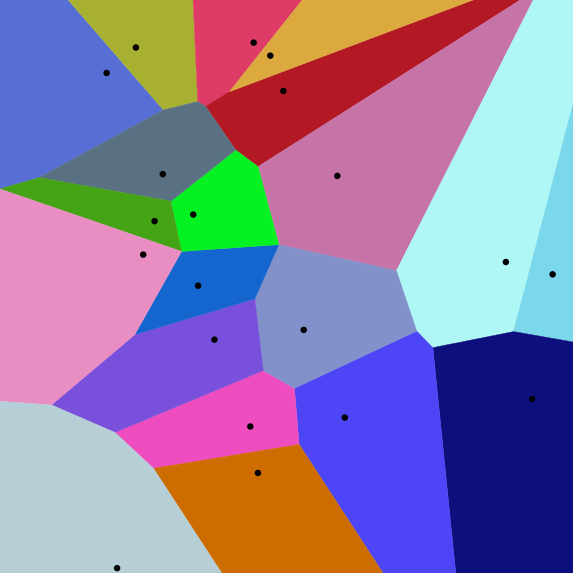
\includegraphics[width=0.3\textwidth]{./Images/Euclidean_Voronoi_diagram.png}
                \caption{Voronoi diagram with Euclidean distance metric}
            \end{figure}
        \end{center}
        \begin{center}
            \begin{figure}[H]
                \centering
                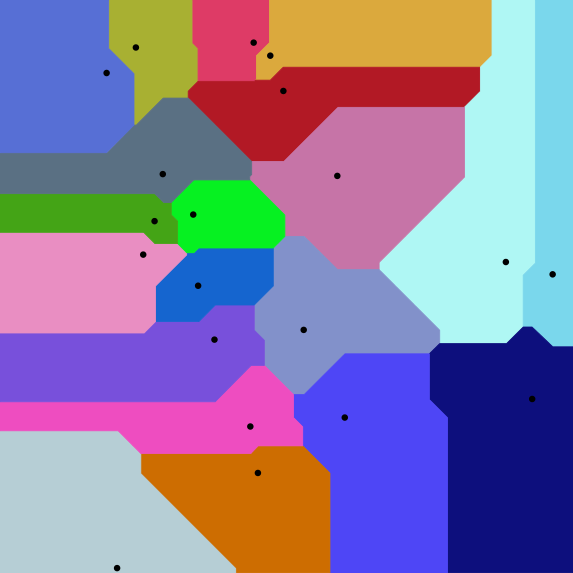
\includegraphics[width=0.3\textwidth]{./Images/Manhattan_Voronoi_Diagram.png}
                \caption{Voronoi diagram with Manhattan distance metric}
            \end{figure}
        \end{center}
    \end{multicols}

Recall that autoencoders performs a mapping of the input space $\mathbb{H}^n$ into a lower-dimensional space $\mathbb{H}^p$ and then back to the original space. The mapping is done by two functions $A$ and $B$ that are learned from the data. The mapping is done in two steps:
\[
    x \xrightarrow{B} h \xrightarrow{A} y
\]

\begin{theorem}
    \textbf{Fixed layer solution}: if the $A$ mapping is fixed , then the optimal mapping $B^*$ is given by $B^*(x) = h_i$ for any $x$ in $\mathcal{C}_i = \mathcal{C}^{Vor}(A(h_i))$. Conversely, if $B$ is fixed, then the optimal mapping $A^*$ is given by $A^*(h_i) = \text{Majority}\left[\mathcal{X} \cap B^{-1}(h_i)\right]$ 
\end{theorem}
\begin{proof}
    Assume first that $A$ is fixed . Then for each of the $2^p$ possible Boolean vectors $h_1, \dots, h_{2^{p}}$ of the hidden layer, $A(h_1), \dots, A(h_{2^p})$ provide $2^p$ points (centroids) in the hypercube $\mathbb{H}^n$. One can build the corresponding Voronoi partition by assigning each point of $\mathbb{H}^n$ to its closest centroid, breaking ties arbitrarily, thus forming a partition of $\mathbb{H}^n$ into $2^p$ corresponding clusters $\mathcal{C}_1, \dots, \mathcal{C}_{2^p}$, with $\mathcal{C}_i = \mathcal{C}^{Vor}(A(h_i))$. The optimal mapping $B^*$ is then given by $B^*(x) = h_i$ for any $x$ in $\mathcal{C}_i$.

    If we consider the input-output layers to have a cardinality of 4 and the hidden layer to have a cardinality of 2, then this would mean that there would be $2^2 = 4$ centroids given by the $A$ mapping in the space $\mathbb{H}^4$ showed in figure:

        \begin{figure}[H]
            \centering
            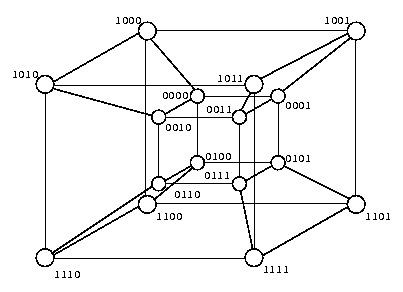
\includegraphics[width=0.5\textwidth]{./Images/Hypercube4Dimensions.png}
            \caption{Hypercube in 4 dimensions}
        \end{figure}
    So, the Voronoi partition would be the partition of the hypercube into 4 regions using as metric the Hamming distance, i.e. the number of edges that need to be crossed to go from one point to each centroid.\\

    Conversely, assume that $B$ is fixed. Then for each of the $2^p$ possible Boolean vectors $h_1, \dots, h_{2^{p}}$ of the hidden layer, let $B^{-1}(h_i) = \{x \in \mathbb{H}^n : B(x) = h_i\}$. To minimize the reconstruction error, $A^*$ must map $h_i$ onto a point $y$ of $\mathbb{H}^n$ minimizing the sum of Hamming distances to points in $\mathcal{X} \cap B^{-1}(h_i)$. By Lemma 3.1 the minimum is realized by the component-wise majority vector $A^*(h_i) = \text{Majority}[\mathcal{X} \cap B^{-1}(h_i)]$, breaking ties arbitrarily. Note that this solution minimizes the distortion on the training set. The generalization or total distortion however, is minimized by $A^*(h_i) = \text{Majority}[B^{-1}(h_i)]$. In some situations, one may have the additional constraint that the output vector must belong to the training. With this additional constraint the optimal solution is $A^*(h_i)$ should be the vector $\mathcal{X}$ that is closest to the vector $\text{Majority}[\mathcal{X} \cap B^{-1}(h_i)]$. 
\end{proof}

\section{Clustering complexity on the hypercube}
\subsection{Brief recap on computational complexity}
Recall that $\mathcal{P}$ is the class of problems that can be \textit{solved} in polynomial time by a deterministic Turing machine, and $\mathcal{NP}$ is the class of problems for which a solution can be \textit{verified} in polynomial time by a deterministic Turing machine. The class $\mathcal{NP}$ is the class of problems that can be solved non-deterministically in polynomial time. A problem is:
\begin{itemize}
    \item \textbf{$\mathcal{NP}$-complete} if it is in $\mathcal{NP}$ and every problem in $\mathcal{NP}$ can be reduced to it in polynomial time
    \item \textbf{$\mathcal{NP}$-hard} if there is a $\mathcal{NP}$-complete problem that can be reduced to it in polynomial time
\end{itemize}
An example of an $\mathcal{NP}$-complete problem is the Boolean satisfiability problem (SAT), which is the problem of determining whether a given Boolean formula can be satisfied by assigning truth values to its variables. If it could be solved in polynomial time, then every problem in $\mathcal{NP}$ could be solved in polynomial time because every problem in $\mathcal{NP}$ can be reduced to SAT in polynomial time.

\subsection{Clustering complexity}
In this section, we briefly review some results on clustering complexity and then prove that the hypercube clustering decision problem is in general NP-complete. 

% missing some details

A graph is cubical if it is the subgraph of some hypercube $\mathbb{H}^d$ for some $d$ (\citep{harary1988cubical}; \citep{livingston1988embeddings}). Although deciding whether a graph is cubical is $\mathcal{NP}$-complete \citep{afrati1985complexity}, there is a theorem (\citep{havel1972b}) providing a necessary and sufficient condition for a graph to be cubical. A graph $G(V,E)$ is cubical and embeddable in $\mathbb{H}^d$ if and only if it is possible to color the edges of $G$ with $d$ colors such that:
\begin{enumerate}
    \item All edges incident with a common vertex are of different color
    \item In each path of $G$, there is some color that appears an odd number of times
    \item In each cycle of $G$, no color appears an odd number of times
\end{enumerate} 
\begin{theorem}
    Consider the following hypercube clustering problem:
    \begin{itemize}
        \item \textbf{Input:} $m$ binary vectors $x_1, \dots, x_m$ of length $n$ and an integer $k$
        \item \textbf{Output:} $k$ binary vectors $c_1, \dots, c_k$ of length $n$ (the centroids) and a function $f$ from $\{x_1, \dots, x_m\}$ to $\{c_1, \dots, c_k\}$ that minimizes the distortion 
        \[
            E = \sum_{t=1}^m \Delta(x_t, f(x_t))    
        \]
        Where $\Delta$ is Hamming distance.
    \end{itemize}
    The hypercube clustering decision problem $\mathcal{NP}$-hard when $k \sim m^\epsilon$ $(\epsilon > 0)$
\end{theorem}
\begin{proof}
    To sketch the reduction, we start from the problem of clustering $m$ points in the plane $\mathbb{R}^2$ using cluster centroids and the $L_1$ distance, which is $\mathcal{NP}$-complete (\citep{megiddo1984complexity}) by reduction from 3-SAT (\citep{garey1979computers}) when $k \sim m^\epsilon$ $(\epsilon > 0)$ (see also \citep{mahajan2012planar}, \citep{vattani2009hardness}). Without any loss of generality, we can assume that the points in these problems lie on the vertices of a square lattice. Using the theorem in \citep{havel1972b}, one can show that a $n \times m$ square lattice in the plane can be embedded in a hypercube $\mathbb{H}^{m+n}$. 
    Example:
    \begin{multicols}{2}
    \begin{center}
                % 4x2 Lattice with different shaped lines
        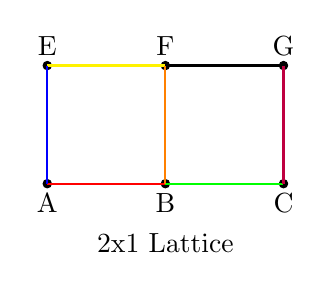
\begin{tikzpicture}[scale=1.5]
            % Draw the grid points
            \filldraw[black] (0,0) circle (1pt) node[anchor=north] {A};
            \filldraw[black] (1,0) circle (1pt) node[anchor=north] {B};
            \filldraw[black] (2,0) circle (1pt) node[anchor=north] {C};
            %\filldraw[black] (3,0) circle (1pt) node[anchor=north] {D};

            \filldraw[black] (0,1) circle (1pt) node[anchor=south] {E};
            \filldraw[black] (1,1) circle (1pt) node[anchor=south] {F};
            \filldraw[black] (2,1) circle (1pt) node[anchor=south] {G};
            %\filldraw[black] (3,1) circle (1pt) node[anchor=south] {H};

            % Connect the points with different line styles
            \draw[red,thick] (0,0) -- (1,0); % Solid line
            \draw[green,thick] (1,0) -- (2,0); % Dashed line
            %\draw[dotted, thick] (2,0) -- (3,0); % Dotted line
            \draw[yellow,thick] (0,1) -- (1,1); % Dash-dot line
            \draw[thick] (1,1) -- (2,1); % Solid line
            %\draw[dashed, thick] (2,1) -- (3,1); % Dashed line
            \draw[blue,thick] (0,0) -- (0,1); % Dotted line
            \draw[orange,thick] (1,0) -- (1,1); % Dash-dot line
            \draw[purple,thick] (2,0) -- (2,1); % Solid line
            %\draw[dashed, thick] (3,0) -- (3,1); % Dashed line

            % Label the lattice
            \node at (1, -0.5) {2x1 Lattice};
        \end{tikzpicture}
    \end{center}
    \columnbreak
    \begin{center}
                % 3D Cube with connections following the lattice pattern
        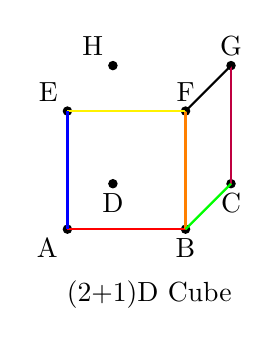
\begin{tikzpicture}[scale=1.5]
            % Draw the vertices of the cube (front and back face)
            \filldraw[black] (0,0,0) circle (1pt) node[anchor=north] {D}; % Front bottom left
            \filldraw[black] (1,0,0) circle (1pt) node[anchor=north] {C}; % Front bottom right
            \filldraw[black] (0,1,0) circle (1pt) node[anchor=south east] {H}; % Front top left
            \filldraw[black] (1,1,0) circle (1pt) node[anchor=south] {G}; % Front top right

            \filldraw[black] (0,0,1) circle (1pt) node[anchor=north east] {A}; % Back bottom left
            \filldraw[black] (1,0,1) circle (1pt) node[anchor=north] {B}; % Back bottom right
            \filldraw[black] (0,1,1) circle (1pt) node[anchor=south east] {E}; % Back top left
            \filldraw[black] (1,1,1) circle (1pt) node[anchor=south] {F}; % Back top right

            % Connect the vertices with corresponding line styles from the lattice
            %\draw[green,thick] (0,0,0) -- (1,0,0); % Solid line (A-B)
            \draw[purple,thick] (1,0,0) -- (1,1,0); % Dashed line (B-F)
            %\draw[purple,thick] (0,1,0) -- (1,1,0); % Dotted line (E-F)
            %\draw[green,thick] (0,0,0) -- (0,1,0); % Dash-dot line (A-E)

            \draw[red,thick] (0,0,1) -- (1,0,1); % Solid line (C-D)
            \draw[orange,thick] (1,0,1) -- (1,1,1); % Dashed line (D-H)
            \draw[yellow,thick] (0,1,1) -- (1,1,1); % Dotted line (G-H)
            \draw[blue,thick] (0,0,1) -- (0,1,1); % Dash-dot line (C-G)

            % Connect the front and back face vertices
            %\draw[blue,thick] (0,0,0) -- (0,0,1); % Solid line (A-C)
            \draw[green,thick] (1,0,0) -- (1,0,1); % Dashed line (B-D)
            %\draw[blue,thick] (0,1,0) -- (0,1,1); % Dotted line (E-G)
            \draw[,thick] (1,1,0) -- (1,1,1); % Dash-dot line (F-H)

            % Label the cube
            \node at (0.5, -0.75, 0.5) {(2+1)D Cube};
        \end{tikzpicture}        
    \end{center}

        \end{multicols}
    
    

    It is easy to check that the $L_1$ or Manhattan distance between any two points on the square lattice is equal to the corresponding Hamming distance in $\mathbb{H}^{m+n}$. This polynomial reduction completes the proof that if the number of cluster satisfies $k = 2^p \sim m^\epsilon$ or equivalently $p \sim \epsilon \log_2 m \sim C \log n$, then the hypercube clustering problem associated with the Boolean autoencoder is $\mathcal{NP}$-hard and the corresponding decision problem is $\mathcal{NP}$-complete. If the numbers $k$ of clusters is fixed and the centroids must belong to the training set, there are only $\binom{m}{k} \sim m^k$ possible choices for the centroids inducing the corresponding Voronoi clusters. This yields a trivial, albeit not efficient, polynomial time algorithm. When the centroids are not required to be in the training set, we conjecture also the existence of polynomial time algorithms by adapting the corresponing theorems in Euclidean space. 
\end{proof}




\end{document}
